\documentclass[11pt]{article}

\usepackage{scrextend}
\usepackage[a4paper, margin = 1.25in,footskip =0.25in]{geometry}
\usepackage{enumitem}
\usepackage{amsmath}
\usepackage{amssymb}
\usepackage{amsthm}
\usepackage{mathtools}
\usepackage{amsmath}
\usepackage{graphicx}
\usepackage{amstext} 
\usepackage{array}


\newcommand{\C}{\mathbb{C}}
\newcommand{\Q}{\mathbb{Q}}
\newcommand{\R}{\mathbb{R}}
\newcommand{\Z}{\mathbb{Z}}

\graphicspath{ {images/} }


\DeclarePairedDelimiter\ceil{\lceil}{\rceil}
\DeclarePairedDelimiter\floor{\lfloor}{\rfloor}

\newcolumntype{L}{>{$}l<{$}} % math-mode version of "l" column type
\begin{document}


\begin{flushleft}
Rowan Lochrin \\
MATH415B - Klaus Lux \\
4/8/18 \\
Homework 9
\end{flushleft}

\section{Gallian}
\begin{description}
\subsection{Chapter 21}

\item[19] Suppose that $p(x) \in F[x]$ and $E$ is a finite extension of $F$. If
	$p(x)$ is irreducible over $F$, and $\deg p(x)$ and $[E:F]$ are
	relatively prime, show that $p(x)$ is irreducible over $E$.

	Let $a$ be a zero of $p(x)$ and let $\deg p(x) = n$. Because $\{1, a, ...
	,a^n \}$ is a basis for $F(a)$ over $F$ by Theorem 20.3 
	$[F(a):F]$ is relatively prime to $[E:F]$. Because $E$ is an
	extension of $F$, $[E(a):E] \leq [F(a):F]$. Also note that
	$$[E(a):F(a)][F(a):F] = [E(a):F] = [E(a):E][E:F] $$
	So $ [F(a):F] $ divides $[E(a):E]$ implying $[F(a):F]=[E(a):E]$, so
	$a \notin E$ and $p$ is irreducible in $E$.
\item[24] Find a splitting field for $x^4 - x^2 - 2$ over $Z_3$.
	$$x^4-x^2-2 = (x^2+1)(x^2-2) = (x+i)(x-i)(x+\sqrt2)(x-\sqrt2)$$
	So $Z_3(i,\sqrt2)$ is a splitting field.
\item[32] Let $f(x)$ and $g(x)$ be irreducible polynomials over a field $F$ and
	let $a$ and $b$ belong to some extension $E$ of $F$. If $a$ is a zero of
	$f(x)$ and $b$ is a zero of $g(x)$, show that  $f(x)$ is
	irreducible over $F(b)$ if and only if $g(x)$ is irreducible
	over $F(a)$.
		
\begin{center}
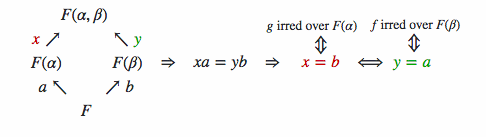
\includegraphics[width=0.75\textwidth]{images/fig1} 
\end{center}

\item[36] 
	Suppose that $a$ is algebraic over a field $F$. Show that $a$ and
	$1+a^{-1}$ have the same degree over $F$.	
	
	We can see that $1+a^{-1} \in F(a)$ and that $a \in F(1+a^{-1})$,
	meaning that $F(a) = F(1+a^{-1}) = F(a,1+a^{-1})$ so
		$$[F(a,1+a^{-1}):F] = [F(a):F] = [F(1+a^{-1}):F]$$
\item[42] Suppose $K$ is an extension of $F$ of degree $n$. Prove that $K$ can
	be written in the form $F(x_1,x_2,...,x_n)$ from some $x_1,x_2,...,x_n$
	in $K$.
	\begin{proof}
	Because $[K:N]$ is finite $K$ must be an algebraic extension of $F$. Let
	$[K:N] = n$, for all $k \in K$ 
		$$k = f_0k_0 + f_1k_1 + ... + f_nk_n$$
	Where $f_1,...,f_n \in F$ and $k_1, ... ,k_n \in K$ we can see that
	$f_0k_0 \in F(k_0)$, so 
		$$k = f_0k_0 + f_1k_1 + ... + f_nk_n \in F(k_0)(k_1)...(k_n) =
		F(k_0,k_1,...,k_n)$$
	\end{proof}

\subsection{Chapter 22}
\item[18]
	Suppose that $[E:Q] = 2$. Show that there is an integer $d$ such that
		$E = Q(\sqrt d)$ where $d$ is not divisible by the square of any
		primes. 
	Let $d = -1$. We can see that $\{1,i\}$ is a basis for $Q(i)$ over $Q$.
\item[24]
	Show that any finite subgroup of the multiplicative group of a field is
	cyclic.

\item[37]
	Let $E$ be the splitting field of $f(x) = x^{p^n}-x$ over $Z_p$. Show
	that the set of zeros of $f(x)$ in $E$ is closed under addition,
	subtraction, multiplication, and division (by nonzero elements). (This
	exercise is referred to in the proof of Therome 22.1)

\end{description}
\section{GAP}
\begin{description}

\item[22.10]

\end{description}
\end{document}
